% Section content template for individual Educative lessons
% This file contains the actual content for a specific section
% Generated from Educative API section content

% Section: Introduction to the Unified Modeling Language
% Section ID: 5905000549318656
% Section Slug: introduction-to-the-unified-modeling-language
% Generated: 2025-12-08T22:21:07.969876

\subsection{What is UML?}\label{what-is-uml}
\\
Models offer us a way to view the system from different angles. However, how exactly does one create a perfect model that meets all our requirements? This scenario is where the Unified Modeling Language (UML) comes into the picture, which is a standard way of visualizing a system's design.
\\
UML is not a programming language but is used to visualize a system's behavior and structure. It is known for providing tools to software engineers and developers that allow them to analyze, design, and develop software systems and model processes. UML is the perfect language to explain the inner workings of the software system to all the stakeholders involved---from an analyst to an author.

\subsection{UML basic notations}\label{uml-basic-notations}
\\
UML is composed of three main building blocks: \textbf{things}, \textbf{relationships}, and \textbf{diagrams}. These three exist at the center of UML and play a key role in producing effective and easily understandable models.
\\
Let's look at these building blocks in detail.
\begin{quote}
\textbf{Note}: We'll look into the relationships and diagrams of building blocks in the upcoming lessons.
\end{quote}
\subsubsection{Things}\label{things}
\\
This building block itself is divided into the following various types:

\begin{itemize}
\item
Structural things
\item
Behavioral things
\item
Grouping things
\item
Annotation things
\end{itemize}
\\
We won't be discussing the grouping and annotation things in detail since their functionalities are pretty much the same as their names. Let 's now explore the structural and behavioral things in detail.
\\
\paragraph{Structural things}\label{structural-things}
\\
The structural things represent a system\textquotesingle s physical aspects, such as a class, object, interface, use case, actor, component, and node. A description of these is provided below:

\begin{enumerate}
\item
\textbf{Class:} The notation represents the attributes and methods of an object.
\end{enumerate}

\begin{figure}[htbp]
 \centering
 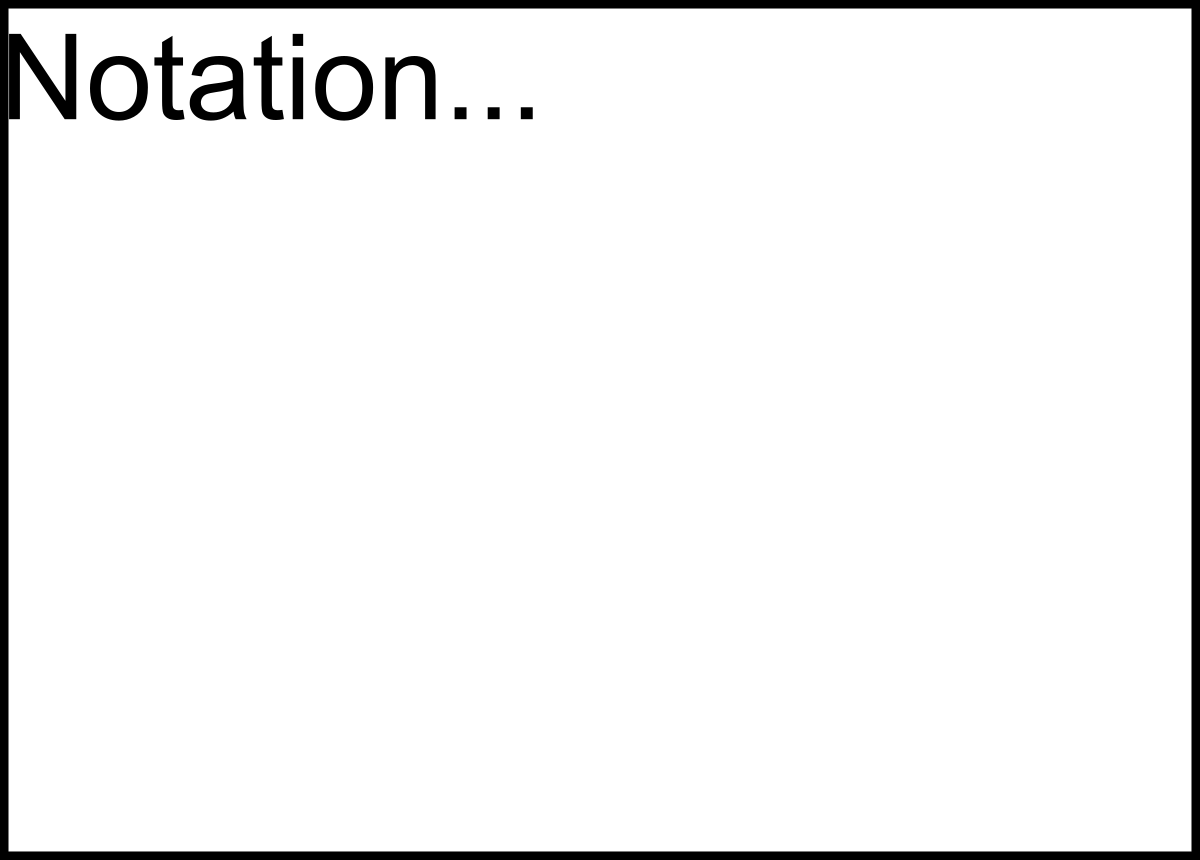
\includegraphics[width=0.15\textwidth]{Images/chapter_3/section_5905000549318656/5338717235707904.png}
 \caption{Class notation}
\end{figure}

\begin{enumerate}
\setcounter{enumi}{1}
\item
\textbf{Object:} This notation refers to the instance of a class.
\end{enumerate}

\begin{figure}[htbp]
 \centering
 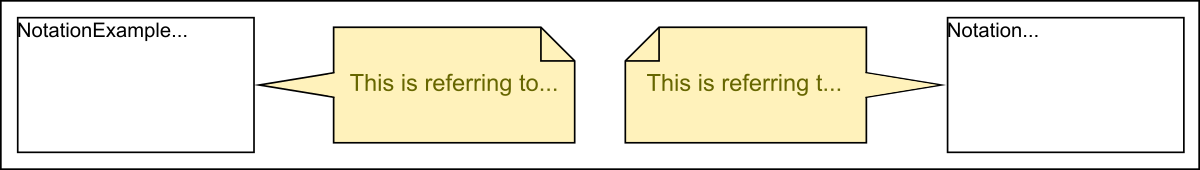
\includegraphics[width=0.5\textwidth]{Images/chapter_3/section_5905000549318656/6002545132830720.png}
 \caption{Object notation}
\end{figure}

\begin{enumerate}
\setcounter{enumi}{2}
\item
\textbf{Interface:} This notation represents the functionality without its implementation.
\end{enumerate}

\begin{figure}[htbp]
 \centering
 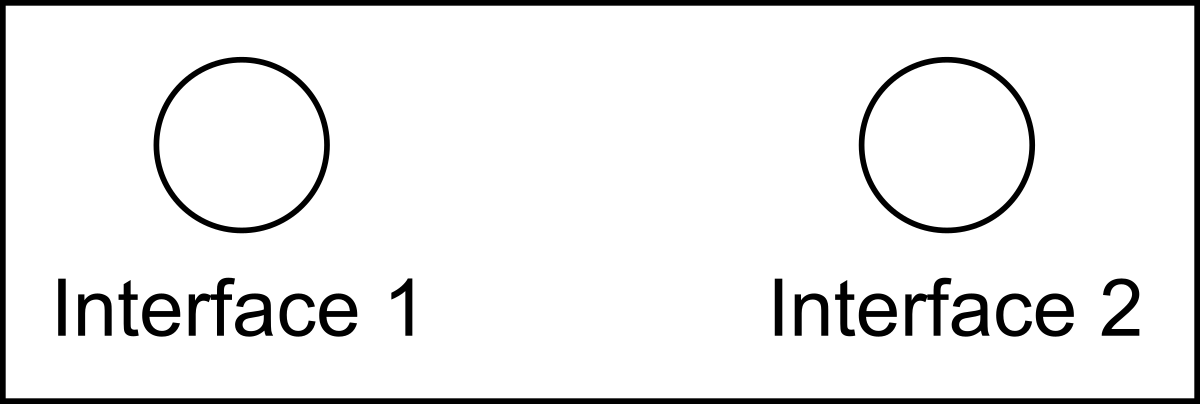
\includegraphics[width=0.15\textwidth]{Images/chapter_3/section_5905000549318656/4964609914306560.png}
 \caption{Interface}
\end{figure}

\begin{enumerate}
\setcounter{enumi}{3}
\item
\textbf{Use case:} This notation describes the users' goals and possible interactions with the system.
\end{enumerate}

\begin{figure}[htbp]
 \centering
 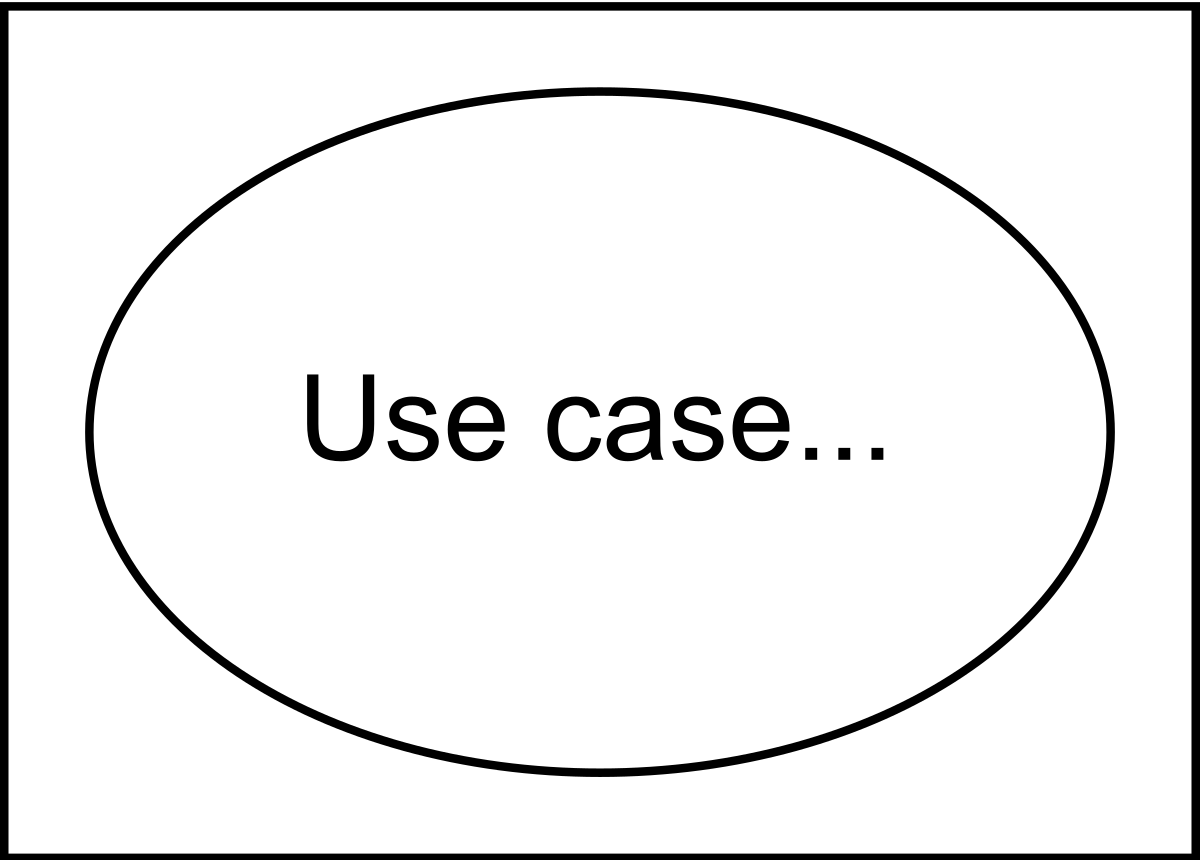
\includegraphics[width=0.15\textwidth]{Images/chapter_3/section_5905000549318656/5634556344664064.png}
 \caption{Use case}
\end{figure}

\begin{enumerate}
\setcounter{enumi}{4}
\item
\textbf{Actor:} This notation represents the entities interacting with the system.
\end{enumerate}

\begin{figure}[htbp]
 \centering
 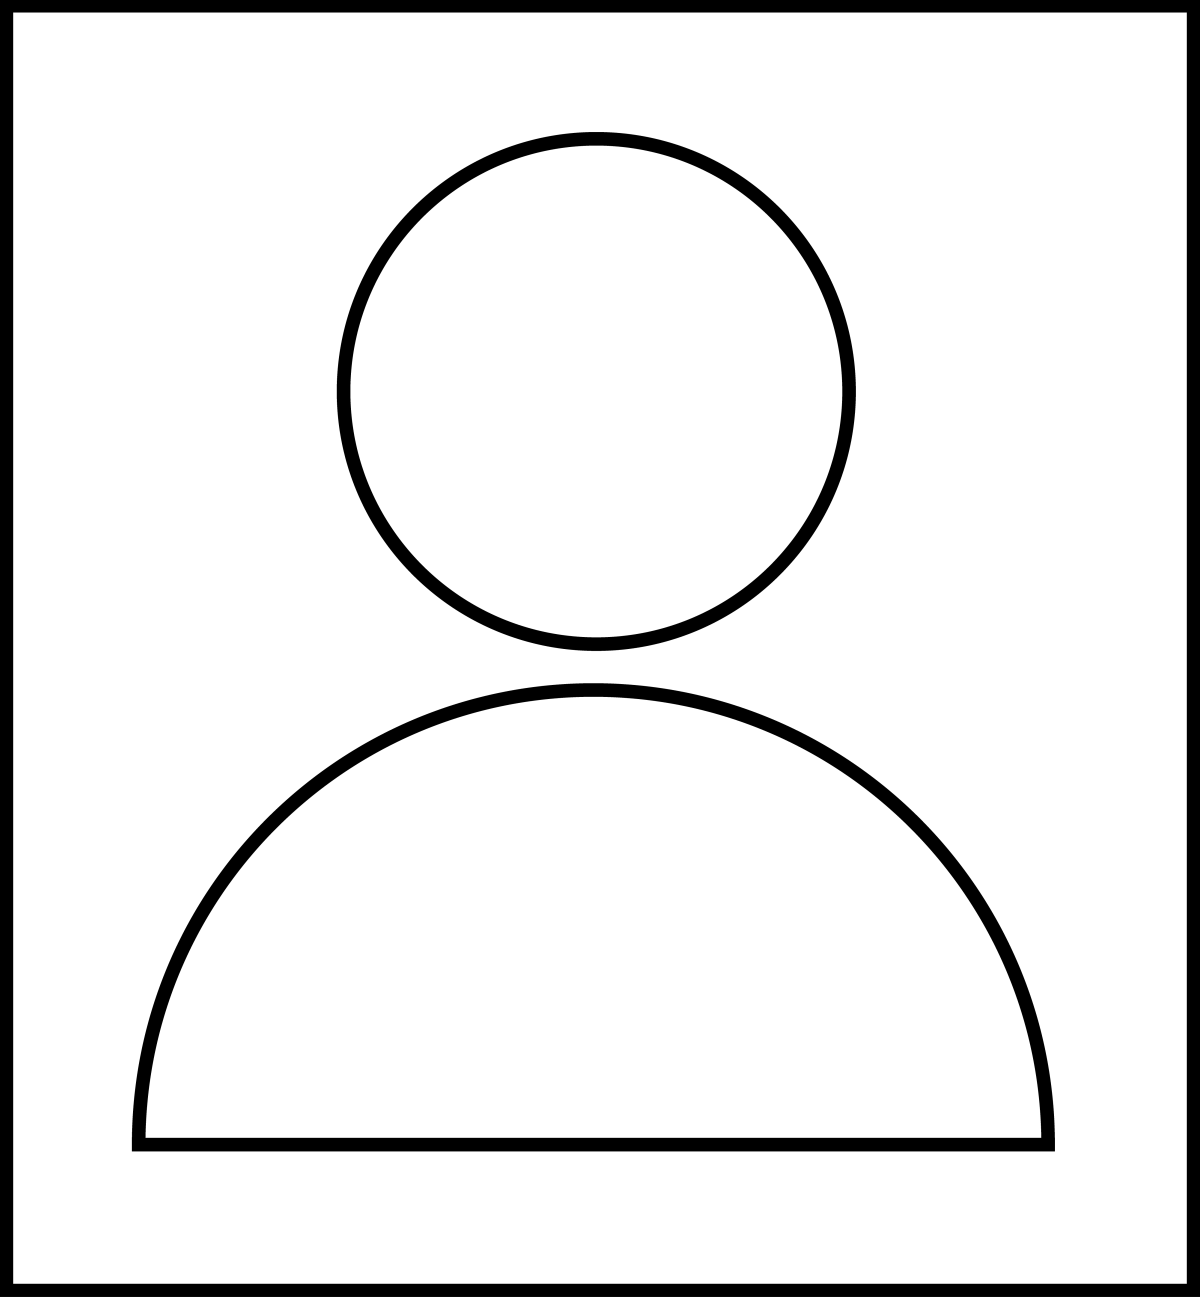
\includegraphics[width=0.15\textwidth]{Images/chapter_3/section_5905000549318656/4774129440129024.png}
 \caption{Actor}
\end{figure}

\begin{enumerate}
\setcounter{enumi}{5}
\item
\textbf{Component:} This notation represents a section of the system.
\end{enumerate}

\begin{figure}[htbp]
 \centering
 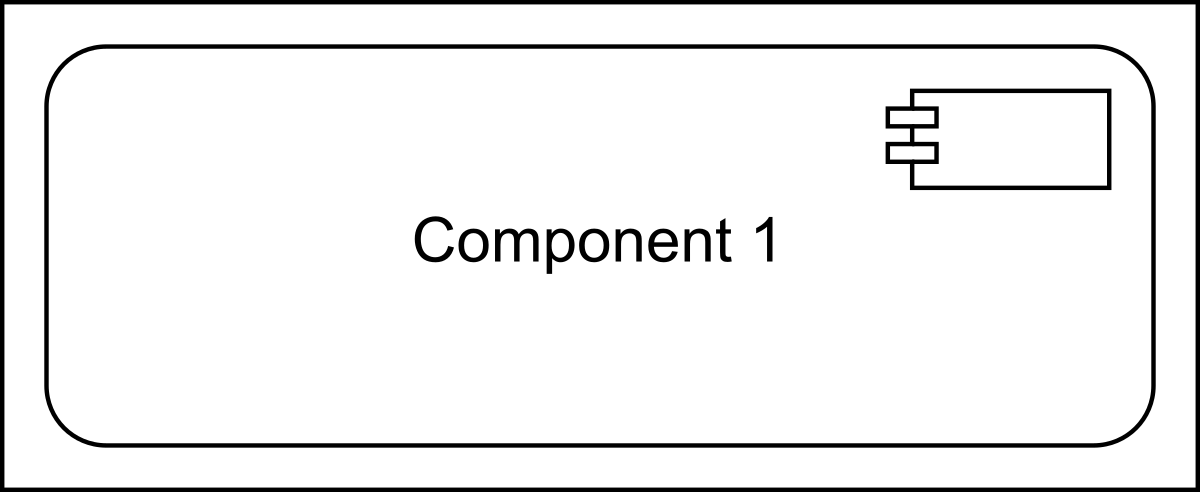
\includegraphics[width=0.15\textwidth]{Images/chapter_3/section_5905000549318656/6096070713278464.png}
 \caption{Component}
\end{figure}

\begin{enumerate}
\setcounter{enumi}{6}
\item
\textbf{Node:} This notation is similar to the component notation, with the difference being that the node notation refers to the physical aspect of a system, such as a server.
\end{enumerate}

\begin{figure}[htbp]
 \centering
 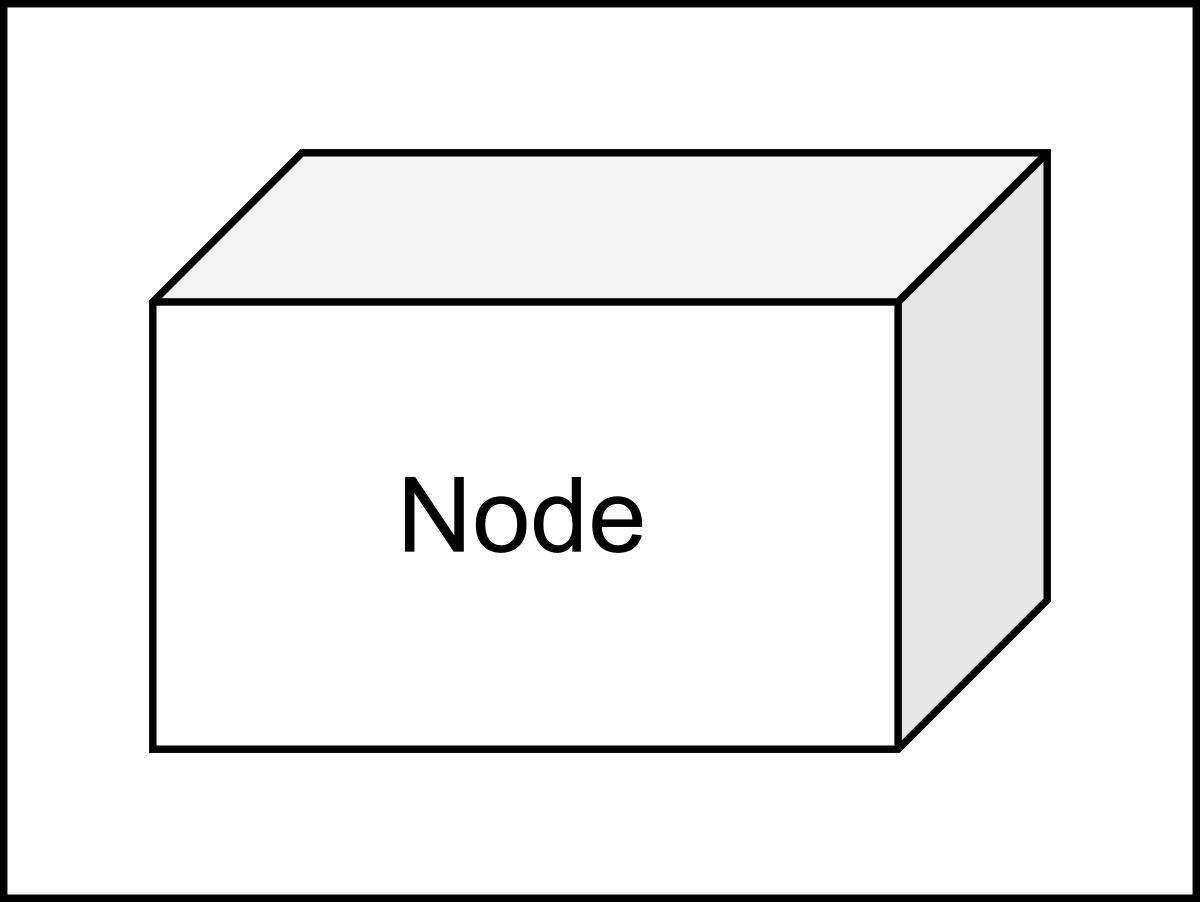
\includegraphics[width=0.15\textwidth]{Images/chapter_3/section_5905000549318656/6346014909005824.png}
 \caption{Node}
\end{figure}

\paragraph{Behavioral things}\label{behavioral-things}
\\
The behavioral things represent the various system\textquotesingle s interactions and functions, such as state machines, activity, and interaction diagrams. The explanation of these behavioral things is given below:
\begin{quote}
\textbf{Note:} We won\textquotesingle t be using state machines in our course, so we won\textquotesingle t go into its details.
\end{quote}
\begin{enumerate}
\item
\textbf{Activity diagrams:} These describe the various interactions performed by different components present in the system.
\end{enumerate}

\begin{figure}[htbp]
 \centering
 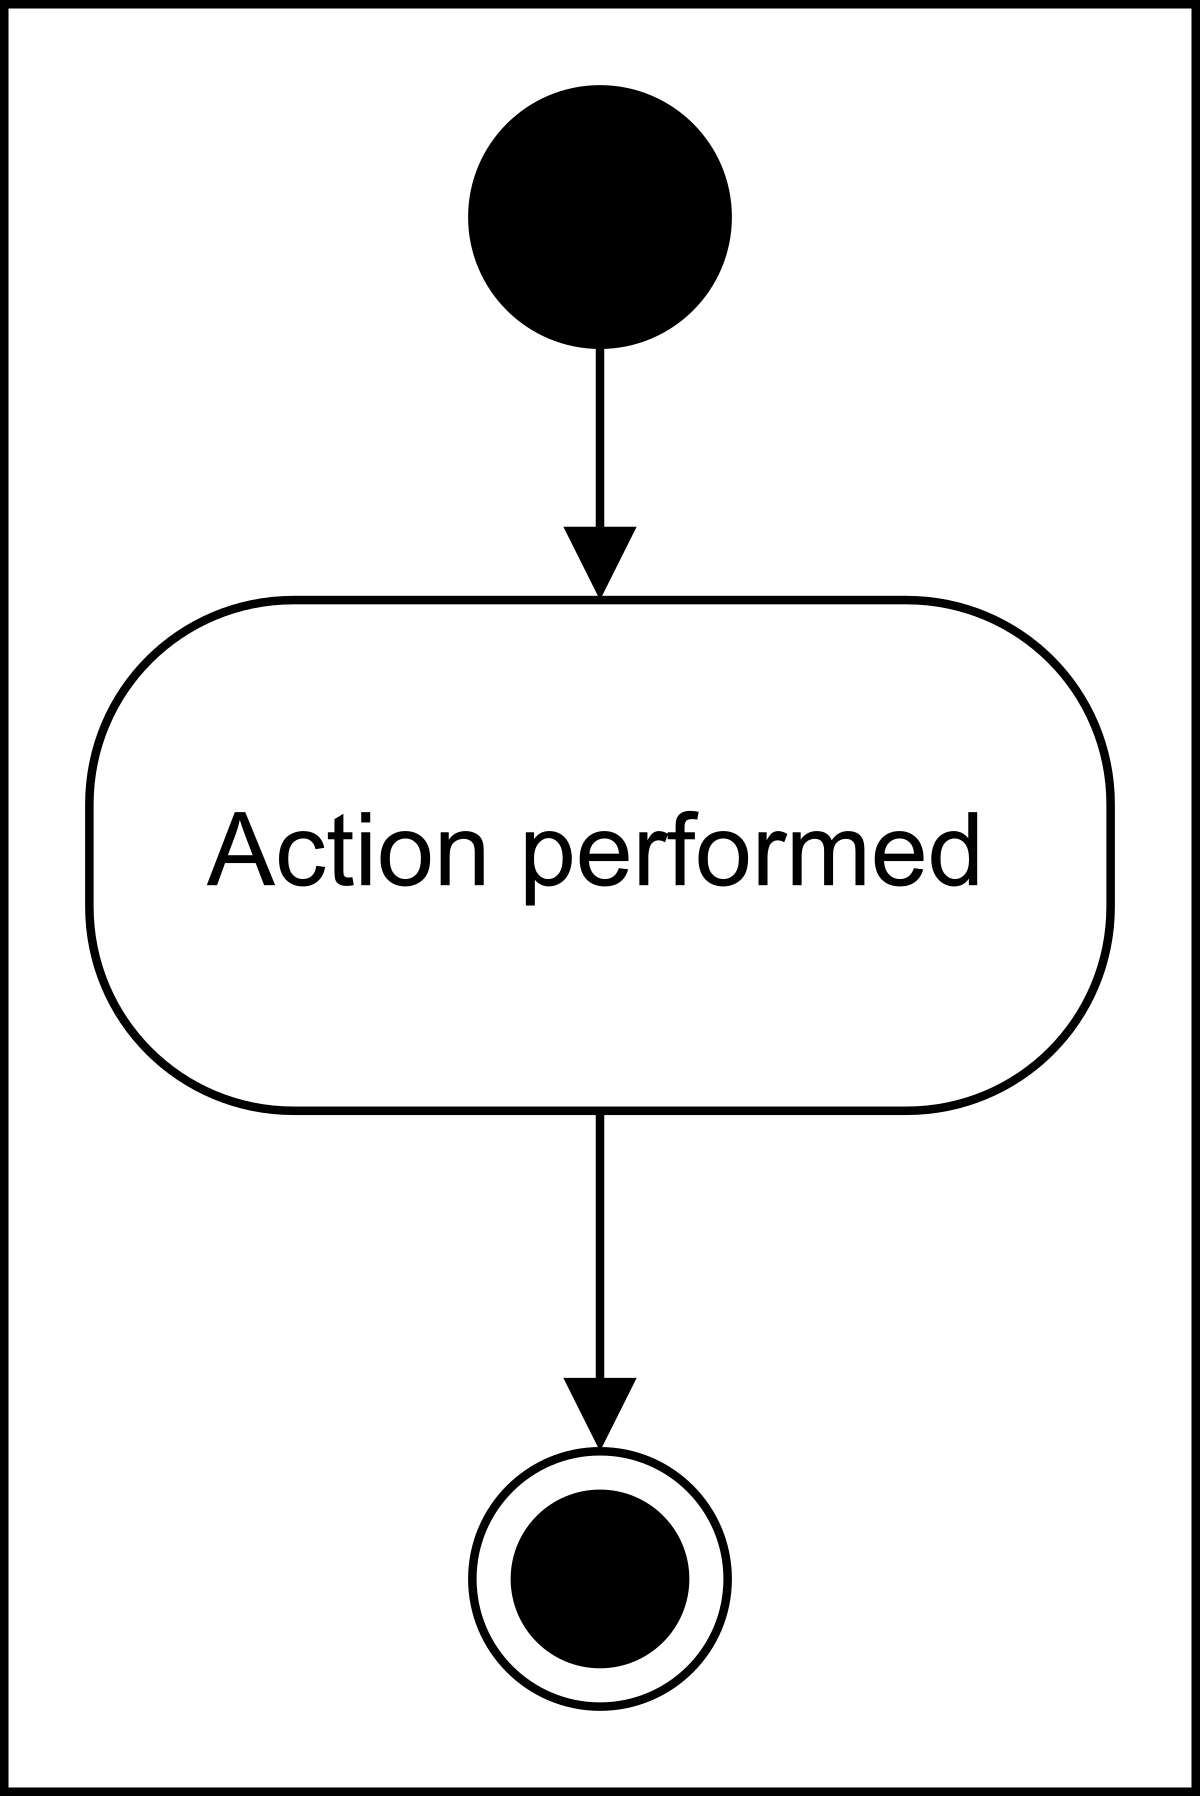
\includegraphics[width=0.15\textwidth]{Images/chapter_3/section_5905000549318656/5374778619985920.png}
 \caption{Activity diagram}
\end{figure}

\begin{enumerate}
\setcounter{enumi}{1}
\item
\textbf{Interaction diagrams:} These diagrams describe the message flow between the different components present in the system.
\end{enumerate}

\begin{figure}[htbp]
 \centering
 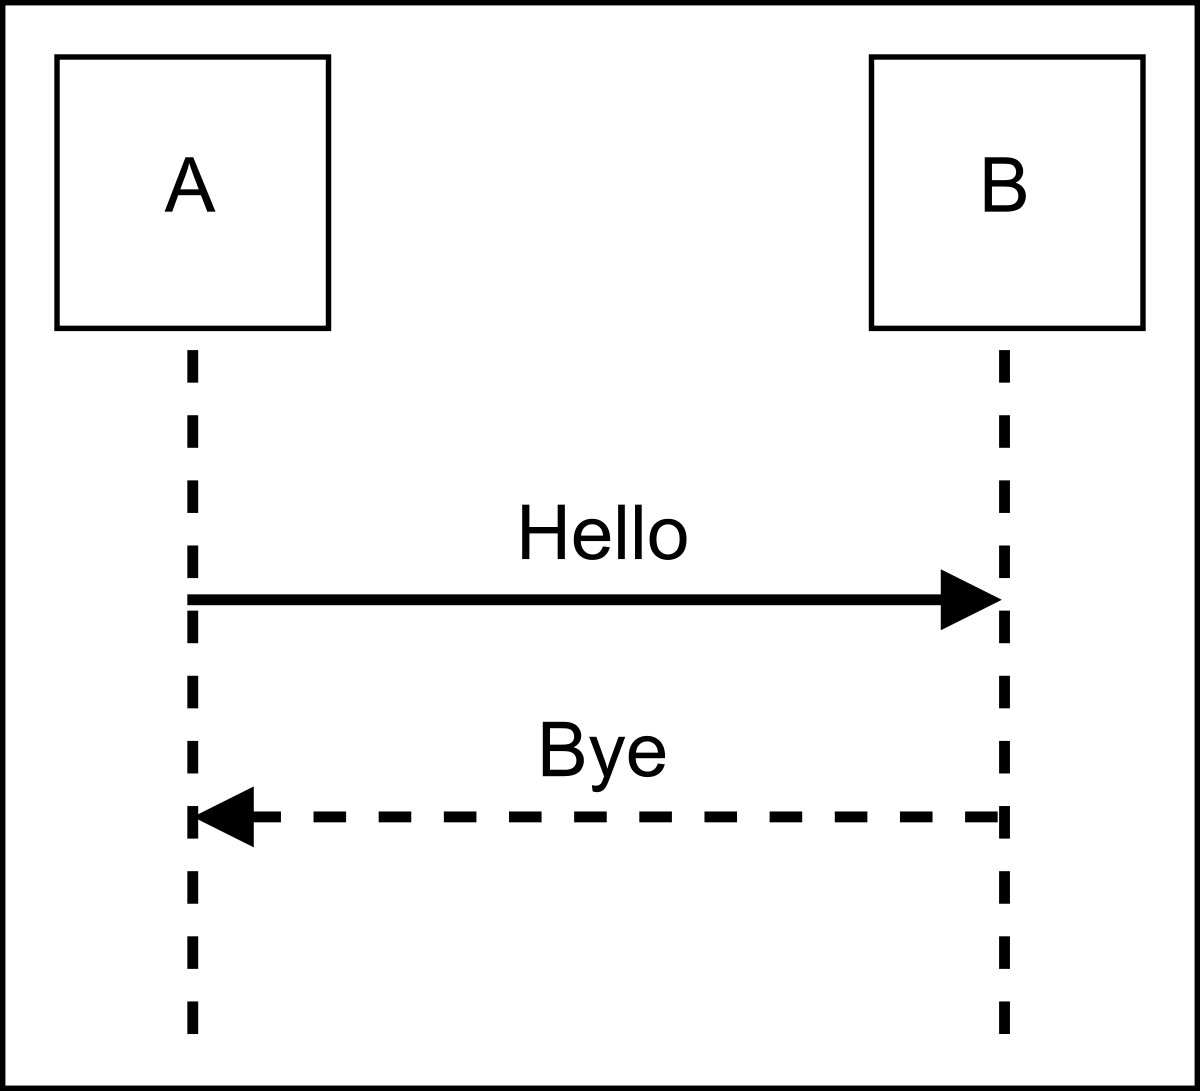
\includegraphics[width=0.15\textwidth]{Images/chapter_3/section_5905000549318656/4673270924443648.png}
 \caption{Interaction diagram}
\end{figure}

\subsection{Benefits of using UML}\label{benefits-of-using-uml}
\\
The following are the advantages of using UML:

\begin{itemize}
\item
It's extraordinarily flexible and easy to understand for all different stakeholders, even those who don't have any technical knowledge.
\item
It's widely used and has a large community, which makes it easier to perform collaborative work among teams.
\item
It has an abundance of tools that helps break complex systems into smaller pieces.
\end{itemize}
\\
Let's explore the various types of UML diagrams in this lesson.

% End of section content